\section{Trigonometry}
\subsection{Common Values and the Unit Circle}
\begin{table}[H]
	\centering
	\renewcommand{\arraystretch}{1.5}
	\begin{tabular}{cccccc}
		\toprule
		$\theta ^ \circ$ & $0^ \circ$ & $30^ \circ$ & $45^ \circ$ & $60^ \circ$ & $90^ \circ$ \\ \midrule
		$\theta ^ c$ & $0$ & $\frac{\pi}{6}$ & $\frac{\pi}{4}$ & $\frac{\pi}{3}$ & $\frac{\pi}{2}$ \\ \midrule
		$\sin \theta$ & $0$ & $\frac{1}{2}$ & $\frac{1}{\sqrt{2}}$ & $\frac{\sqrt{3}}{2}$ & $1$ \\
		$\cos \theta$ & $1$ & $\frac{\sqrt{3}}{2}$ & $\frac{1}{\sqrt{2}}$ & $\frac{1}{2}$ & $0$ \\
		$\tan \theta$ & 0 & $\frac{1}{\sqrt{3}}$ & $1$ & $\sqrt{3}$ & N/D \\ \bottomrule
	\end{tabular}
	\caption{\label{standardvals}Commonly used trigonometric values. Refer the \hyperref[unitcircle]{Unit Circle}}
\end{table}
\begin{figure}[ht]
	\centering
	\includegraphics[scale=0.8]{figures/Unit_circle_angles.pdf}
	\caption{\label{unitcircle} Unit Circle}
\end{figure}

\subsection{Pythagorean Identities}
\begin{align*}
	\sin^2x + \cos^2x &= 1 &  \sec^2 x - \tan^2x &= 1 \\
	 \csc^2 x - \cot^2 x &= 1
\end{align*}

\subsection{Double Angle Formulae}
\begin{align*}
\sin{(2x)} &= 2\sin x\cos x & \tan{(2x)} &= \frac{2\tan x}{1 - \tan^2x} \\
\cos{(2x)} &= 2\cos^2x - 1 \\
&= \cos^2x - \sin^2x \\ &= 1 - 2\sin^2x
\end{align*}

\subsection{Sum and Difference Formulae}
\begin{align*}
&\sin{(x \pm y)} = \sin x\cos y \pm \cos x\sin y &
\cos{(x \pm y)} &= \cos x \cos y \mp \sin x \sin y \\
&\tan{(x \pm y)} = \frac{\tan x \pm \tan y}{1 \mp \tan x \tan y}
\end{align*}
\begin{align*}
&\arcsin x \pm \arcsin y = \arcsin{(x\sqrt{1 - y^2}\pm y\sqrt{1 - x^2})} \\ &\arccos x \pm \arccos y = \arccos{(xy \mp \sqrt{(1-x^2)(1-y^2)})} \\
&\arctan x \pm \arctan y = \arctan{(\frac{x\pm y}{1 \mp xy})}
\end{align*}

\subsection{Sum to Product Formulae}
\begin{align*}
&\sin x + \sin y = 2\sin{\left(\frac{x+y}{2}\right)}\cos{\left(\frac{x-y}{2}\right)} & &\sin x - \sin y = 2\cos{\left(\frac{x+y}{2}\right)}\sin{\left(\frac{x-y}{2}\right)} \\
&\cos x + \cos y = 2\cos{\left(\frac{x+y}{2}\right)}\cos{\left(\frac{x-y}{2}\right)} &
&\cos x - \cos y = -2\sin{\left(\frac{x+y}{2}\right)}\sin{\left(\frac{x-y}{2}\right)}
\end{align*}
\subsection{Product to Sum Formulae}
\begin{align*}
\sin(x + y) \sin(x - y) &= \sin^2x - \sin^2y &
\cos(x + y) \cos(x - y) &=\cos^2x - \sin^2y \\
\end{align*}
\subsection{Laws of Sines and Cosines}
\begin{figure}[H]
	\centering
	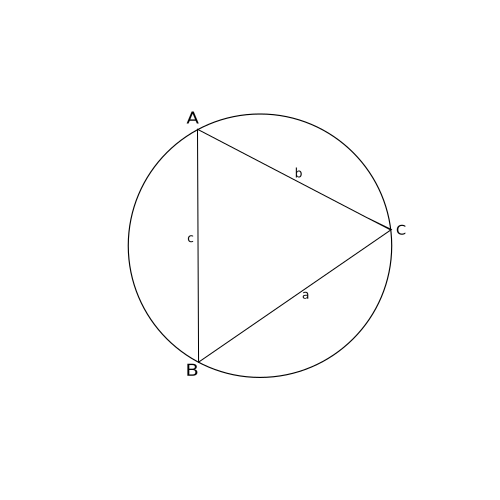
\includegraphics[scale=1]{figures/triangle}
	\caption{\label{triangle}$\Delta ABC$ in a circumscribed circle of circumradius $r$}
\end{figure}
\paragraph{Law of Sines}
$$\frac{\sin A}{a} = \frac{\sin B}{b} = \frac{\sin C}{c} = \frac{1}{2r}$$
\paragraph{Law of Cosines}
\begin{align*}
&a^2 = b^2 + c^2 - 2bc\cos A & &A =\cos^{-1}{\left(\frac{b^2 + c^2 - a^2}{2bc}\right)} \\
&b^2 = a^2 + c^2 - 2ac\cos B & &A =\cos^{-1}{\left(\frac{a^2 + c^2 - b^2}{2ac}\right)} \\
&c^2 = a^2 + b^2 - 2ab\cos C & &C =\cos^{-1}{\left(\frac{a^2 + b^2 - c^2}{2ab}\right)} \\
\end{align*}

\subsection{Inverse Trigonometric Functions}
\begin{align*}
	&\sin^{-1}(-x) =-\sin^{-1}x &   &\cos^{-1}(-x) =\pi-\cos^{-1}x, & &\lvert x\rvert\leq 1 \\
	&\tan^{-1}(-x) =-\tan^{-1}x &   &\cot^{-1}(-x) =\pi-\cot^{-1}x,& &x\in\mathbf{R} \\
	&\csc^{-1}x =\sin^{-1}\left(\frac{1}{x}\right) & &\sec^{-1}x =\cos^{-1}\left(\frac{1}{x}\right),& &\lvert x\rvert\geq1 \\ &\cot^{-1}x =\tan^{-1}\left(\frac{1}{x}\right),& & & &x>0 \\
	&\cot^{-1}x =\pi+\tan^{-1}\left(\frac{1}{x}\right),& & & &x<0 \\
	&\sin^{-1}x+\cos^{-1}x =\frac{\pi}{2},& & &  &\lvert x\rvert\leq1 \\
	&\csc^{-1}x+\sec^{-1}x =\frac{\pi}{2},& & & &\lvert x\rvert\geq1
\end{align*}

\subsection{Trigonometry in the Complex Plane}
\paragraph{Euler's Formula}
$$re^{i\theta} = r(\cos\theta + i\sin\theta)$$
\paragraph{De Moivre's Formula}
$${(\cos\theta + i\sin\theta)}^n = \cos{(n\theta)} + i\sin{(n\theta)}$$
\paragraph{Exponential Definition of Trigonometric Functions}
\begin{align*}
\cos{(ix)} &= \frac{(e^x + e^{-x})}{2} & \sin{(ix)} &= i\frac{(e^x - e^{-x})}{2} & \tan{(ix)} &= i\frac{(e^x - e^{-x})}{(e^x + e^{-x})}
\end{align*}
\paragraph{Exponential Definition of Hyperbolic Functions}
\begin{align*}
\cosh{(x)} &= \frac{(e^x + e^{-x})}{2} & \sinh{(x)} &= \frac{(e^x - e^{-x})}{2} & \tanh{(x)} &= \frac{(e^x - e^{-x})}{(e^x + e^{-x})}
\end{align*}
\paragraph{Relationship between hyperbolic and trigonometric functions}
\begin{align*}
\cosh x &= \cos{ix} & \cos x = \cosh{ix} \\
i\sinh x &= \sin{ix} & i\sin{x} = \sinh{ix}
\end{align*}

\subsection{Hyperbolic Identities}
\begin{align*}
&\cosh^2 x - \sinh^2 x = 1 & &\sech^2x + \tanh^2x = 1 & &\csch^2x + \coth = 1\\
&\sinh{(2x)} = 2\sinh x\cosh x & &\cosh{(2x)} = \cosh^2x + \sinh^2{x} & &\sinh x + \cosh x = e^x \\
\end{align*}

\subsection{Inverse Hyperbolic Functions}
\begin{align*}
\cosh^{-1}x &= \ln{(\sqrt{1 + x^2} + x)} & \sinh^{-1}x &= \ln{(\sqrt{1 + x^2} + x)} \\
\tanh^{-1}x &= \ln{\sqrt{\frac{1 + x}{1 - x}}} \\
&= \frac{1}{2}\ln{\frac{1+x}{1-x}}
\end{align*}
